\chapter{Design und Implementation}
\section{Authentifizierung}
\xxx[@rliebi: kapitel design = IST zustand. hier hat es vergleiche]
In diesem Kapitel werden verscheidene Methoden der Authentifizierung beleuchtet.
\subsection{Herkömmliche Registrierung per E-Mail}
Die herkömmliche Registrierung bietet den Vorteil, dass sie keine Abhängigkeiten zu Dritt-Providern erfordert. So kann sich jeder Benutzer mit einer gültigen E-Mail Adresse einloggen. Ein Nachteil dieser Methode kann sein, dass Dummy-Adressen verwendet werden können und so ein registrierter Benutzer nicht wirklich Authentifiziert ist.
\subsection{oAuth2}
oAuth2 hat einen anderen Ansatz. Sociale Netzwerke bieten sich an, um mit den Login-Daten des bereits bestehenden Accounts in einem solchen ein Account bei opendatahub zu erstellen. So ist der Benutzer der sich registriert bereits authentifizert und es kann davon ausgegangen werden, dass es sich wirklich um diesen handelt. Die häufigkeit von``Fake-Profilen'' wird dadurch reduziert.

\subsection{Cookie-Based-Authentication}
Bei der Cookie-Based-Authentifizierung wird eine Session-ID auf der Seite des Clients in einem Server-Side Cookie gespeichert. Dieses wird mit jedem Request an den Server übermittelt. So kann der Server davon ausgehen, dass es sich beim Client um den Inhaber der Session ID handelt.

\subsection{Token-Based-Authentication}
Ein neuerer Ansatz, ist es, einen Signierten Token im Header jedes Requests der zum Server geht mitzusenden. Vorteile dieser Variante sind bestechend:
\begin{description}
  \item[Cross-Domain / CORS]
  Cookies und CORS spielt nicht so sauber zwischen mehreren Domains. Ein Token basierter Ansatz erlaubt es AJAX Aufrufe an jeden Server mit jeder Domain zu veranlassen, weil die Informationen im HTTP Header liegen.
  \item[Stateless (Server-Side-Scalability)]Es wird kein Session-Store benötigt. Der Token enthält alle Benutzerinformationen der Rest des `States' liegt im Local Storage auf der Client-Side.
  \item[Decoupling] Man ist nicht an ein Authentifizierungs-Schema gebunden. Der Token kann überall generiert werden, sprich die API kann von überall her aufgerufen werden.
  \item[Mobile-Ready]Cookies sind in nativen mobilen Apps böse.
  \item[CSRF]Cross-Site Requests stellen kein Problem dar. Es gibt kein Authentication Cookie, das wiederverwendet werden könnte.
  \item[Standard]Es gibt bereits einen Standard. (\gls{JWT})
\end{description}
\begin{figure}[H]
    \centering
    \includegraphics[width=\linewidth]{fig/cookie-token-auth}
    \caption{Vgl. Cookie vs. Token Auth}
    \label{fig:pd:cookie-token-auth}
\end{figure}
\section{Architektur}
\xxx
Daten-Lieferanten liefern ihre Daten per Web-Interface oder REST-API. Diese Daten werden in der Datenbank gespeichert und im Web-Interface angezeigt. Daten-Nutzer rufen diese Daten wieder über das Web-Interface oder per REST-API ab. 

Dritt-Entwickler können eigene Komponenten entwickeln und beisteuern, wie in \cref{fig:pd:arch-overview} zu sehen ist:
\begin{description}
\item[Parser] nehmen Daten entgegen und bereiten sie zur Weiterverarbeitung auf
\item[Formatter] formatieren Daten in das vom Benutzer gewünschte Format
\end{description}

\begin{figure}[H]
    \centering
    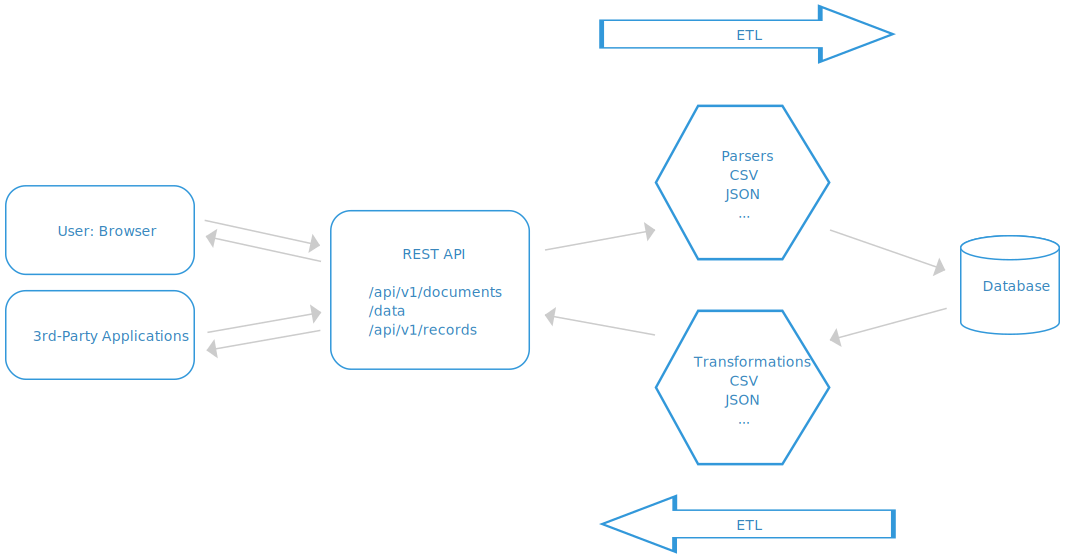
\includegraphics[width=\linewidth]{fig/ODH-Architecture-Overview}
    \caption{Grobe Architektur-Übersicht}
    \label{fig:pd:arch-overview}
\end{figure}

\subsection{Komponenten und Packages}

\begin{figure}[H]
    \centering
    \includegraphics[width=\linewidth]{fig/packages}
    \caption{Python Packages}
    \label{fig:pd:pypackages}
\end{figure}

\subsection{Klassen}


\subsection{Sequenzdiagramm}


\section{Transformationssprache ODHQL}

\subsection{Syntax}

Die Syntax von \acs{odhql} orientiert sich stark an SELECT aus ANSI SQL.

Eine formale Beschreibung der Transformations-Sprache ist in \cref{app:odhql-syntax} zu finden.

\subsection{Unterstützte Features}

\cref{tab:pd:transformation-lang-impl} beschreibt die unterstützten Features:
\mytable{lX}{
  \textbf{Anforderung} & \textbf{Beschreibung}\\
  \midrule
  \textbf{Mapping} & Felder können mit oder ohne Alias angegeben werden. Falls kein Alias vorhanden ist wird der Feldname beibehalten. Es ist möglich, Sonder- und Leerzeichen zu verwenden, indem der Feldname in doppelten Anführungszeichen geschrieben wird. \\
  \textbf{Default-Werte} & Unterstützt werden Integer, Float, sowie Strings (in einfachen Anführungszeichen). \\
  \textbf{Joins} & Es muss immer mindestens eine Datenquelle angegeben werden. Falls mehr verwendet werden sollen muss mindestens eine Join-Bedingung vorhanden sein (es werden mehrere Join-Bedingungen unterstützt, jedoch nur per ``and''-Verknüpung). Neben Inner Joins werden auch Left, Right und Full Outer Joins unterstützt. \\
  \textbf{Filter/Prädikate} & Vorhandene Filter beinhalten: ``is null'', ``in (...)'', relationale Operatoren wie ``='', ``<'', etc, Prädikate und ``like `regex'\ '' (letzteres ist eine Abweichung von ANSI SQL, welches eine separate Syntax für Like-Filter hat) \\
  \textbf{Erweiterbare Funktionen} & Alle Funktionen werden über eine Function Registry in Python aufgerufen und können daher einfach erweitert werden. \\
  \textbf{Sortierung} & Es kann eine Order By-Klausel angegeben werden. Falls Unions verwendet werden muss die Order By-Klausel am Ende angegeben werden, nicht pro Query. \\
  \textbf{Unions} & Mehrere Queries können per Union zusammengefügt werden. Die Implementation entspricht dem UNION ALL aus SQL, es findet also keine Deduplizierung statt. \\
}{Durch \acs{odhql} implementierte Features}{pd:transformation-lang-impl}

Jede Transformation definiert eine Liste von Feldern oder Werten, sowie mindestens eine Datenquelle. 

\subsection{Beispiele}
Folgende Items sind in der Feld-Liste erlaubt:
\begin{description}
\item[Feld] Name des Feldes, mit dem Namen oder Alias der Datenquelle als Präfix. Feld-Namen und Aliases können in doppelten Anführungszeichen geschrieben werden, z.B. wenn Sonder- oder Leerzeichen verwendet werden sollen. Zu beachten ist, dass Feld-Namen immer einen Präfix brauchen, auch ausserhalb der Feld-Liste.
\begin{src}{sql}
a.beschreibung, a.geom as geometry, a."Zentroid X [m]"
\end{src}
\item[Wert] Integer, Float, Boolean, Null oder String in einfachen Anführungszeichen. Es muss zwingend ein Alias angegeben werden. 
\begin{src}{sql}
1 as one, 3.14 as pi, false as active, 'sun' as local_star
\end{src}
\item[Funktion] Ein Funktionsaufruf besteht aus einem Namen sowie einer Liste von Argumenten in runden Klammern. Funktionsaufrufe können verschachtelt werden.
\begin{src}{sql}
 cast(a.pi, 'float') as pi,
 concat('POINT(', cast(v0.x, 'string'), ' ', cast(v0.y, 'string'), ')')) as geometry
\end{src}
\end{description}

Datenquellen können per Join verknüpft werden.
\begin{src}{sql}
  from "Gebäude" as geb join Strassen as str on geb.str_id = str.id
\end{src}

Unterstützt werden Inner Join, Left, Right und Full Outer Join. Dabei wird jeweils die einfachste Syntax\footnote{\texttt{join}, \texttt{left join}, \texttt{right join} und \texttt{full join}.} verwendet.

Als Filter können folgende Ausdrücke verwendet werden:
\begin{description}
\item[Relationale Operatoren] Unterstützt werden die Operatoren `=', `!=', `<', `>', `<=', `>='.
\begin{src}{sql}
a.nr > 4, a.active = false
\end{src}
\item[Like] Anders als bei SQL verwendet der Like-Operator von \acs{odhql} implementationsbedingt Reguläre Ausdrücke (Python Syntax\footnote{Siehe \url{https://docs.python.org/2/library/re.html\#regular-expression-syntax}}).
\begin{src}{sql}
a.beschreibung like 'Z[uü]rich', a.beschreibung not like 'Z[uü]rich'
\end{src}
\item[In] Sucht den Ausdruck in einer Liste von Elementen.
\begin{src}{sql}
a.nr in (3, 4, 5), a.nr not in (2, 6, 7)
\end{src}
\item[Null-Check] Prüft, ob ein Ausdruck Null (bzw. None) ist.
\begin{src}{sql}
a.optional_field is null, a.mandatory_field is not null
\end{src}
\end{description}

Die Resultate mehrerer Queries werden mit Union zusammengehängt. Dies verhält sich wie ``union all'' in SQL, d.h. es findet keine Deduplizierung der Daten statt.
\begin{src}{sql}
  select a.description, a.geometry from A as a
   union
  select b.description, b.geometry from B as b
\end{src}
Zu beachten ist, dass die Feld-Listen der Queries kompatibel sein müssen.
\newline

\subsection{Abstrakter Syntax-Baum (AST)}
Der ODHQL-Parser analysiert die Abfrage in Text-Form und wandelt diese in einen Abstrakten Syntax Baum (AST) um. Dieser wird anschliessend vom Interpreter verwendet, um die Transformation auf die Daten anzuwenden.

\cref{fig:pd:odhql-ast-toplevel} zeigt die Toplevel-Struktur des Abstrakten Syntax-Baums.
\begin{figure}[H]
\centering
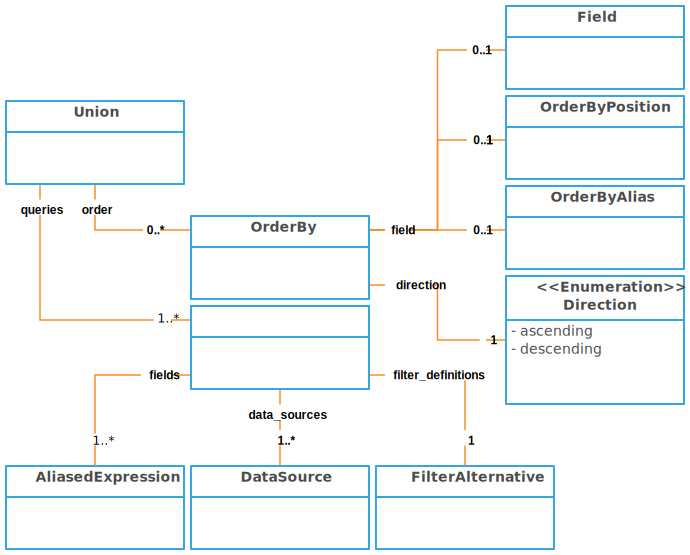
\includegraphics[width=0.8\linewidth]{fig/odhql-ast-union.pdf}
\caption{AST: Unions}
\label{fig:pd:odhql-ast-toplevel}
\end{figure}

Die in \cref{fig:pd:odhql-ast-expressions} beschriebenen Ausdrücke repräsentieren Felder, Werte, Funktionsaufrufe, etc.
\begin{figure}[H]
\centering
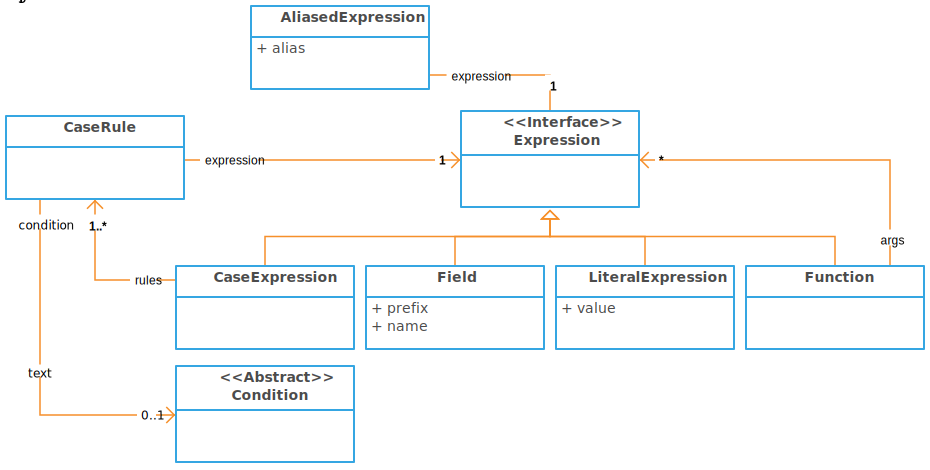
\includegraphics[width=0.8\linewidth]{fig/odhql-ast-expression.pdf}
\caption{AST: Ausdrücke}
\label{fig:pd:odhql-ast-expressions}
\end{figure}

\cref{fig:pd:odhql-ast-datasources} zeigt auf, wie Datenquellen repräsentiert werden.
\begin{figure}[H]
\centering
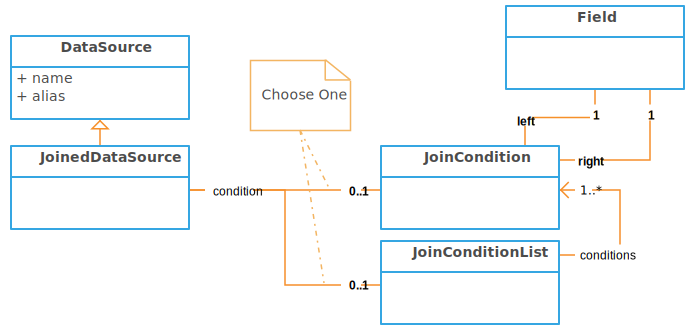
\includegraphics[width=0.8\linewidth]{fig/odhql-ast-datasources.pdf}
\caption{AST: Datenquellen}
\label{fig:pd:odhql-ast-datasources}
\end{figure}

Filter werden wie in \cref{fig:pd:odhql-ast-filter} beschrieben dargestellt.
\begin{figure}[H]
\centering
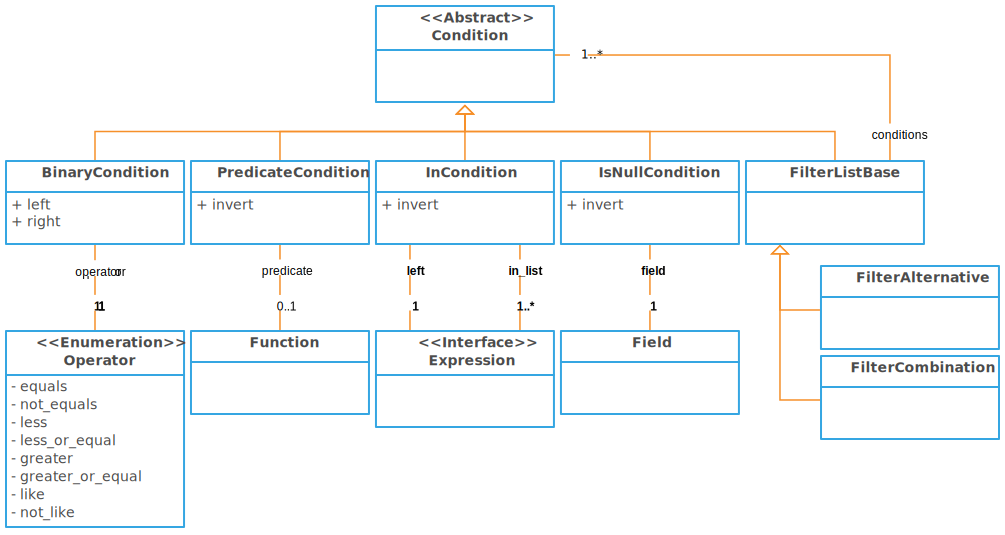
\includegraphics[width=0.8\linewidth]{fig/odhql-ast-filter.pdf}
\caption{AST: Filter}
\label{fig:pd:odhql-ast-filter}
\end{figure}

\subsection{Interpreter}
Mit Pandas und NumPy ist bereits eine API für viele SQL-ähnliche Operationen wie Selektion, Joins und diverse String- und Geometriefunktionen (GeoPandas Erweiterung) vorhanden. Die Herausforderung bei der Entwicklung des Interpreters liegt somit einerseits in einer performanten und möglichst fehlerfreien Ausführung sowie der Erweiterbarkeit durch eigene Funktionen.

\begin{figure}[H]
\centering
\includegraphics[width=0.6\linewidth]{fig/odhql-flow.pdf}
\caption{High-level Ablauf der Abfrage-Interpretation}
\label{fig:pd:odhql-flow}
\end{figure}


\subsection{Funktionen}
Die Funktionen der \acs{odhql} wurden möglichst erweiterbar implementiert. Jede Funktion ist als Python Klasse zu implementieren, welche von der Klasse \path{VectorizedFunction} erben und die Methode \path{apply} zu implementieren hat. Durch die Vererbung und der zugrundeliegenden Python-Metaklasse wird die neue Funktion automatisch registriert und ist sofort mit dem Klassennamen verfügbar. Der Name kann jedoch durch das statische Attribut \path{name} auch explizit gesetzt werden. Die Anzahl Funktionsparameter werden vom Interpreter bzw. von der Execution-Engine der Funktionen via Reflection sichergestellt. Für die Überprüfung der Argumente ist jede Funktion selbst zuständig. Die Parent-Klasse bietet jedoch bereits einige Assertion-Methoden z.B. für Datentypen, Listen und Geometrien.

Ein Beispiel einer solchen Funktion ist in \cref{src:pd:odhql-function} ersichtlich. Hierbei wird nach der Überprüfung der Argumente direkt an die Pandas-Methode \path{str.pad} weiterdelegiert.


\begin{srclst}[label=src:pd:odhql-function]{python}{Beispiel-Implementation der ODHQL-Funktion \texttt{PAD()}}
from hub.odhql.functions.core import VectorizedFunction

class Pad(VectorizedFunction):
    name = 'PAD'

    def apply(self, strings, width, side):
        self.assert_str('string', strings)
        self.assert_in('side', side, ['left', 'right', 'both'])
        self.assert_int('width', width)
        return strings.str.pad(width, side)
\end{srclst}


\section{Caching}
Aufgrund der Entscheidung alle Daten Verlustfrei im Originalformat zu speichern sowie der Verwendung von In-Memory Tabellen-artigen Datenstrukturen, muss sichergestellt werden, dass nicht bei jeder Operation die Originaldaten von Format-Parser neu eingelesen werden müssen.

Aus diesem Grund wurde ein dreistufiges Caching-Konzept für die gesamte Applikation implementiert. Es werden die Caching-Mechanismen von Django mit eingen Modifikationen/Erweiterungen verwendet. Aus diesem Grund können die Caching-Backends jederzeit durch beliebige von Django Unterstützte Backends wie z.B. Memcached, Filesystem, etc. verwendet werden.

\subsection{Caches}

\xxx[ref]
\begin{figure}[H]
\centering
\includegraphics[width=\linewidth]{fig/caching.pdf}
\caption{Übersicht der Caches}
\label{fig:pd:caches}
\end{figure}

\xxx[ref]
\mytable{lX}{
  \textbf{Cache} & \textbf{Beschreibung}\\
  \midrule
  Level 1 & Der Level 1 Cache ist ein In-Memory Cache der Applikation und sehr kurzlebig (\SI{60}{\second}). Dieser wird hauptsächlich verwenden um Zwischenresultate wie Formatkonversionen oder Resultate einer Abfrage zu speichern, damit der Benutzer im Webfrontend die Daten sofort mittels Pagination anschauen kann.\\

  Level 2 & Im Cache zweiter Stufe werden hauptsächlich Daten des Level 3 Caches für mehrere Minuten zwischengespeichert um den Overhead der Abfrage inkl. potenziellem Transfer mehrerer Megabytes sowie Deserialisierung der Python Objekte aus der Datenbank zu vermeiden.\\

  Level 3 & Im persistenten Cache werden eingelesene Dateien im intermediären Format (d.h. DataFrame Objekte) sowie gespeicherte Transformationen ohne Online-Datenquellen persistiert.\\
}{Beschreibung der Caches}{pd:caches}

\subsection{Invalidierung}
\xxx[fscala: cache key]

\section{Format-Unterstützung}
\subsection{Unterstützte Formate}
\cref{tab:pd:formats} beschreibt die implementierten Formate.

\mytable{lX}{
  \textbf{Format} & \textbf{Implementiert via}\\
  \midrule
  CSV (inkl. GeoCSV) & (Geo)Pandas \\
  Excel (xls, xlsx) & Pandas \\
  GML & ogr2ogr \\
  GeoJSON & GeoPandas \\
  GeoPackage & GeoPandas \\
  Interlis 1 & ogr2ogr \\
  Interlis Modell (ili) & custom \\
  JSON & Pandas \\
  KML  & fastkml, custom \\
  ESRI Shapefile & GeoPandas \\
  WFS (nur Parser) & ogr2ogr \\
  XML & custom \\
}{Beschreibung der implementierten Formate}{pd:formats}
\xxx[figure out footnotes in that env]
% \footnote{deaktiviert, siehe \cref{sec:pd:format-gdal-problems}}

GeoPandas verwendet (via Fiona) ebenfalls GDAL.

\subsubsection{Probleme mit GDAL}\label{sec:pd:format-gdal-problems}
Für einen grossen Teil der Formate wird GDAL verwendet, entweder via GeoPandas/Fiona oder direkt per ogr2ogr. 

Folgende GDAL-Versionen stehen zum aktuellen Zeitpunkt zur Verfügung:
\begin{itemize}
\item 1.10.1
\item 1.11.0 - 1.11.2
\item 2.0.0beta1
\end{itemize}

Die Entwicklungsumgebung bestand aus einer virtuellen Maschine mit Ubuntu 14.04 LTS, für welches ein GDAL-Package in Version 1.10.1 vorhanden ist. 

Der Betreuer wünschte jedoch, dass wenn möglich Unterstützung für das relativ neue Format GeoPackage eingebaut wird. GDAL 1.10.1 unterstützt GeoPackage nicht.

Im Versuch, diese Unterstützung einzubauen wurde GDAL selbst kompiliert. Dem Betreuer waren Probleme mit GDAL 1.11.2 bekannt, weswegen 1.11.1 gewählt wurde.

In Tests wurden folgende Probleme gefunden:
\begin{itemize}
\item In GDAL 1.11.0 bis 2.0.0beta1 führt der Versuch, nach Interlis 1 zu konvertieren, zu einem Segmentation Fault. Das Problem wurde vom Betreuer weitergemeldet. In aktuellen nightly-Versionen soll dies behoben sein - dies wurde nicht verifiziert.
\item Der GeoPackage-Treiber wurde in GDAL 1.11.0 hinzugefügt. Leider kann er in dieser Version nur als unausgereift bezeichnet werden:
  \begin{itemize}
  \item Layer-Namen werden ohne Bereinigung oder Maskierung als Tabellen-Namen verwendet, was zu Exceptions seitens SQLite führt.
  \item Wenn die Ursprungs-Daten bereits eine Spalte namens ``fid'' beinhalten, bricht die Konvertierung ab wegen doppelter Spalten-Namen, da der Treiber diese selbst nochmals hinzugeneriert.
  \item Reine Daten-Tabellen werden nicht unterstützt. Diese sind zwar nicht Bestandteil des reinen GeoPackage-Standards, können aber mit Extended GeoPackage realisiert werden. Dies ist in GDAL erst ab Version 2.0.0 möglich.
  \end{itemize}
\end{itemize}

GeoPackage-Support wurde in GDAL 2.0.0 massiv verbessert. Diese Version ist bei Abschluss der Arbeit jedoch noch in der Beta-Phase, weshalb diverse unserer Abhängigkeiten noch nicht dazu kompatibel sind.

\xxx[Reword. I'm srsly bad at this o.O]
\begin{decision}[label=dec:pd:gdal-version]{GDAL-Version}
Zum Abgabe-Zeitpunkt sind folgende GDAL-Versionen verfügbar: 1.10.1, 1.11.0 - .2 und 2.0.0beta1.

Wegen Problemen mit mehreren Treibern entfallen die Versionen 1.11.x.

Version 2.0.0beta1 entfällt wegen mangelnder Unterstützung in unseren Abhängigkeiten.

Daher wird vorerst GDAL 1.10.1 eingesetzt.
\end{decision}

\subsubsection{Interlis 2}
Aufgrund von Problemen mit dem Format-Support in ogr2ogr wurde in Absprache mit dem Betreuer entschieden, Unterstützung für Interlis 2 nicht zu implementieren. Siehe dazu das Sitzungsprotokoll vom 15.04.2015.

\subsubsection{Erweiterung}
Die Unterstützung für neue Formate kann relativ einfach hinzugefügt werden. Dazu müssen Subklassen für folgende Python-Klassen erstellt werden:

\begin{description}
\item[hub.formats.core.Format] Dient zur Identifikation des Formats von Datenquellen (z.B. Dateien)
\item[hub.formats.core.Formatter] Erhält DataFrames und produziert Dateien, welche der Benutzer herunterladen kann.
\item[hub.formats.core.Parser] Erhält Daten (aus Dateien, WFS, ...) und produziert DataFrames, welche von ODH weiterverwendet werden können.
\end{description}

Für die Implementation via ogr2ogr stehen im Modul hub.formats.geobase Hilfsklassen zur Verfügung.

Durch Vererbung und die verwendete Python-Metaklasse wird das neue Format automatisch registriert und kann sofort verwendet werden.

Ein Beispiel ist in \cref{src:pd:format-example} zu sehen. Darin wird die Unterstützung für ESRI Shapefile implementiert. Der Formatter verwendet hierzu die Hilfsklasse GeoFormatterBase, der Parser jedoch direkt GeoPandas.

\begin{srclst}[label=src:pd:format-example]{python}{Beispiel-Implementation der Format-Unterstützung für ESRI Shapefile}
import geopandas as gp
import os

from hub.formats import Format, Parser
from hub.formats.geobase import GeoFormatterBase
from hub.utils import ogr2ogr

if 'ESRI Shapefile' in ogr2ogr.SUPPORTED_DRIVERS:
    class Shapefile(Format):
        label = 'ESRI Shapefile'
        ogr_format = ogr2ogr.SHP

        description = """
        Ein ursprünglich für die Firma ESRI entwickeltes Format für Geodaten.
        """

        extension = 'shp'

        @classmethod
        def is_format(cls, file, *args, **kwargs):
            return file.extension == 'shp'

    class ShapefileFormatter(GeoFormatterBase):
        targets = Shapefile,

        supported_types = {'Point', 'LineString', 'LinearRing', 'Polygon', 'MultiPoint'}

        @classmethod
        def format(cls, dfs, name, format, *args, **kwargs):
            return super(ShapefileFormatter, cls).format(dfs, name, format, 'ESRI Shapefile', 'shp', *args, **kwargs)

    class ShapefileParser(Parser):
        accepts = Shapefile,

        @classmethod
        def parse(cls, file, format, *args, **kwargs):
            with file.file_group.on_filesystem() as temp_dir:
                return gp.read_file(os.path.join(temp_dir, file.name), driver='ESRI Shapefile')
\end{srclst}


\section{API}
Die Webapplikation kommuniziert mit dem Server über ein \gls{rest} \gls{api}.

\subsection{Konzepte}
Folgende Konzepte werden von mehreren Endpunkten verwendet und werden daher separat aufgelistet.

\subsubsection{Paging} \label{sec:pd:api-paging} 
Paging ermöglicht das limitieren der Anzahl Resultate, welche eine Abfrage liefert. Die Einträge pro Seite werden mit dem Parameter \texttt{count} gesteuert, die Seite mit \texttt{page}.

\subsubsection{Suche} \label{sec:pd:api-search} 
Für die Suche werden folgende Parameter verwendet:
\mytable{lX}{
  \textbf{Parameter} & \textbf{Beschreibung}  \\
  \midrule
  \textbf{filter[name]} & Filtert anhand des Namens \\
  \textbf{filter[description]} & Filtert anhand der Beschreibung \\
  \textbf{filter[search]} & Filtert sowohl mit Namen als auch mit der Beschreibung \\
  \textbf{filter[mineOnly]} & Liefert nur Dokumente, die dem eingeloggten Benutzer zugeordnet sind \\
}{Such-Parameter}{pd:api-search}

\subsubsection{Sortierung} \label{sec:pd:api-sort}
Sortiert die Resultate der Anfrage. Dazu kann der Parameter \texttt{sorting[key]=asc|desc} verwendet werden, mit folgenden Werten als \texttt{key}: \texttt{name}, \texttt{description}, \texttt{private}, \texttt{owner} und \texttt{created\_at}.

\paragraph{Preview} \label{sec:pd:api-preview}
Liefert eine Vorschau der Daten. Enthalten ist der Unique Name, welcher in Abfragen verwendet werden kann, eine Liste der Felder und deren Typen sowie ein paar Daten-Zeilen. Die Anzahl der gelieferten Daten-Zeilen kann per Paging gesteuert werden (siehe \cref{sec:pd:api-paging}).

\begin{srclst}{json}{Preview für ein Dokument}
[  
   {  
      "type":"preview",
      "unique_name":"ODH4_Bahnhoefe",
      "parent":"4",
      "types":{  
         "TYPE":"BIGINT",
         "fid":"TEXT",
         "CNTRYNAME":"TEXT",
         "DUP_NAME":"TEXT",
         "PROV1NAME":"TEXT",
         "LEVEL":"BIGINT",
         "geometry":"GEOMETRY",
         "NATION":"BIGINT",
         "CONURB":"TEXT",
         "name":"TEXT"
      },
      "url":"http://beta.opendatahub.ch/api/v1/document/4/preview/",
      "columns":[ "TYPE", "fid", "geometry", "DUP_NAME", "PROV1NAME", "LEVEL", "CNTRYNAME", "NATION", "CONURB", "name" ],
      "data":[  
         {  
            "TYPE":"3",
            "fid":"F0",
            "CNTRYNAME":"Switzerland",
            "DUP_NAME":"N",
            "PROV1NAME":"Tessin",
            "LEVEL":"10",
            "geometry":"POINT (45.90247783251107 76645.7742365048)",
            "NATION":"41",
            "CONURB":"NULL",
            "name":"Chiasso Rail"
         },
         ...
      ],
      "count":1781,
      "name":"Bahnhoefe"
   }
]
\end{srclst}

\subsubsection{Download} \label{sec:pd:api-download}
Fordert einen Download der Daten an. Das gewünschte Format wird mit dem Parameter \texttt{fmt} angegeben. Gültige Werte sind die von \cref{sec:pd:api-format} gelieferten Namen. Ohne Format-Angabe werden die Original-Daten geliefert.

Hinweis: Dokumente können nicht als ganzes heruntergeladen werden. Stattdessen müssen die File Groups für diesen Zweck verwendet werden.

\subsection{Root - GET /api/v1/}
Als Prefix für die \gls{api} URLs wird \url{/api/v1/} verwendet, was eine spätere versionierte Erweiterung erlaubt.
\begin{figure}[H]
\centering
\includegraphics[width=\linewidth]{fig/api-root}
\caption{API: Übersicht}
\label{fig:pd:api-root}
\end{figure}

Da für die Implementation des \gls{api} die Django-Erweiterung \texttt{rest\_framework}\footnote{\url{http://www.django-rest-framework.org/}} verwendet wurde, kann die API gut auch manuell ausprobiert werden. Dabei ist zu beachten, dass die Schrägstriche am Ende der URLs nicht optional sind.

\subsection{Konfiguration - GET /api/v1/config/}
Gibt die für den HTML5 Client notwendigen Konfigurationsinformationen zurück.

\begin{srclst}{json}{Beispielantwort für GET /api/v1/config/}
{
  "GITHUB_PUBLIC": "8ef558ed3fb0f5385da5", 
  "FACEBOOK_PUBLIC": "401520096685508", 
  "PACKAGE_PREFIX": "ODH", 
  "TRANSFORMATION_PREFIX": "TRF"
}
\end{srclst}

\subsection{Liste der unterstützten Formate - GET /api/v1/format/} \label{sec:pd:api-format}
Liefert die Liste der unterstützten Formate. Neue Formate erscheinen automatisch, sobald sie registriert sind, vorausgesetzt dass ein Formatter für das Format existiert.

\begin{srclst}{json}{Beispielantwort für GET /api/v1/format/}
[
    {
        "name": "JSON", 
        "label": "JSON", 
        "description": "JavaScript Objekt-Notation. Nützlich zur Wiederverwendung in Webapplikationen.", 
        "example": "", 
        "extension": "json"
    }, 
    {
        "name": "GML", 
        "label": "GML", 
        "description": "Geometry Markup Language (GML) ist ein Dateiformat zum Austausch von Geodaten.", 
        "example": "", 
        "extension": "gml"
    }, 
    ...
]
\end{srclst}

\subsection{Packages}
``Package'' wird als Überbegriff für Dokumente, welche von Nutzern hochgeladen wurden, und Transformationen verwendet. Packages haben Attribute wie Name und Beschreibung, können eine Vorschau erzeugen und der Benutzer kann einen Download anfordern.

\subsubsection{Package-Liste - GET /api/v1/package/}\label{sec:pd:api-package-list}
Liefert eine Liste der Packages.

\begin{srclst}{json}{Beispielantwort für GET /api/v1/package/}
{
    "count": 37, 
    "next": "http://beta.opendatahub.ch/api/v1/package/?page=2", 
    "previous": null, 
    "results": [
        {
            "id": 1, 
            "url": "http://beta.opendatahub.ch/api/v1/package/1/", 
            "name": "Test mockaroo.com.csv", 
            "description": "Testdaten (Originalformat: CSV)", 
            "private": false, 
            "owner": {
                "id": 1, 
                "username": "testuser", 
                "first_name": "", 
                "last_name": ""
            }, 
            "created_at": "2015-06-01T12:35:31.480135Z", 
            "type": "document", 
            "preview": "http://beta.opendatahub.ch/api/v1/document/1/preview/", 
            "template": false
        }, 
        {
            "id": 2001, 
            "url": "http://beta.opendatahub.ch/api/v1/package/2001/", 
            "name": "TROBDB: Baustellen Februar 2015", 
            "description": "TROBDB: Baustellen Februar 2015", 
            "private": false, 
            "owner": {
                "id": 1, 
                "username": "testuser", 
                "first_name": "", 
                "last_name": ""
            }, 
            "created_at": "2015-06-01T12:35:45.794037Z", 
            "type": "transformation", 
            "preview": "http://beta.opendatahub.ch/api/v1/transformation/2001/preview/", 
            "template": false
        },
        ...
    ]
}
\end{srclst}

Dieser Endpunkt unterstützt Paging (\cref{sec:pd:api-paging}), Suche (\cref{sec:pd:api-search} und Sortierung (\cref{sec:pd:api-sort}).

\subsubsection{Package-Details - GET /api/v1/package/<id>/}\label{sec:pd:api-package-details}
Liefert die Details zu einem Package. Dies sind grundsätzlich die selben Informationen wie in der Package-Liste, jedoch um einige weitere Details ergänzt.

Die Antwort sieht unterschiedlich aus, je nach dem ob das Package ein Dokument (\cref{pd:api-package-document}) oder eine Transformation (\cref{pd:api-package-transformation}) ist.

\begin{srclst}[label=pd:api-package-document]{json}{Beispielantwort für ein Dokument}
{
    "id": 4, 
    "url": "http://beta.opendatahub.ch/api/v1/document/4/", 
    "name": "Test Bahnhoefe.gml, Bahnhoefe.gfs, Bahnhoefe.xsd", 
    "description": "Testdaten (Originalformat: GML)", 
    "file_groups": "http://beta.opendatahub.ch/api/v1/document/4/filegroup/", 
    "private": false, 
    "owner": {
        "id": 1, 
        "username": "testuser", 
        "first_name": "", 
        "last_name": ""
    }, 
    "created_at": "2015-06-01T12:35:32.241407Z", 
    "preview": "http://beta.opendatahub.ch/api/v1/document/4/preview/", 
    "type": "document"
}
\end{srclst}

\begin{srclst}[label=pd:api-package-transformation]{json}{Beispielantwort für eine Transformation}
{
    "id": 2001, 
    "url": "http://beta.opendatahub.ch/api/v1/transformation/2001/", 
    "name": "TROBDB: Baustellen Februar 2015", 
    "description": "TROBDB: Baustellen Februar 2015", 
    "transformation": "SELECT t.\"Federführende_Stelle\" as userid,
           substring(t.Bauarbeiten, 1, 100) as title,
           t.Bauarbeiten as description,
           to_char(to_date(concat(extract(t.Dauer, '^((?:\\\\d\\\\d?\\\\.){2})'), nvl(extract(t.Dauer, '(\\\\d{4}) -'), extract(t.Dauer, '(\\\\d{4})$'))), '%d.%m.%Y'), '%Y-%m-%d') as trob_start, -- add year from end date if not present
           to_char(to_date(extract(t.Dauer, '- ([\\\\d\\\\.]+)'), '%d.%m.%Y'), '%Y-%m-%d') as trob_end,
           null as trob_interval,
           'both' as direction,
           null as diversion_advice,
           'CH' as country,
           t.Bauarbeiten as reason,
           t.Strecke as object_name,
           'street' as object_type,
           'closed' as trob_type,
           ST_SetSRID(ST_GeomFromText(CONCAT('POINT(', CAST(t.\"Zentroid X [m]\", 'text'), ' ',CAST(t.\"Zentroid Y [m]\", 'text'), ')')), 21781) as geometry
           from \"ODH8_Baustellen Februar 2015\" as t", 
    "private": false, 
    "owner": {
        "id": 1, 
        "username": "testuser", 
        "first_name": "", 
        "last_name": ""
    }, 
    "data": "http://beta.opendatahub.ch/api/v1/transformation/2001/data/", 
    "is_template": false, 
    "preview": "http://beta.opendatahub.ch/api/v1/transformation/2001/preview/", 
    "referenced_file_groups": "http://beta.opendatahub.ch/api/v1/transformation/2001/filegroups/", 
    "referenced_transformations": "http://beta.opendatahub.ch/api/v1/transformation/2001/transformations/", 
    "type": "transformation"
}
\end{srclst}

\paragraph{File Groups} Die \texttt{file\_group}-Url liefert die Liste der File Groups, die zu diesem Dokument gehören. Siehe auch \cref{sec:pd:api-filegroups}.

\paragraph{Preview} Die Preview-Url liefert eine Vorschau der Daten im Package. Siehe auch \cref{sec:pd:api-preview}.

\paragraph{Referenced File Groups/Transformations} Dies sind Urls für File Groups bzw. Transformations, welche in dieser Transformation verwendet wurden.

\paragraph{Template} Templates sind abstrakte Transformationen, welche als Vorlage für konkrete Transformationen dienen. Für Templates kann keine Vorschau erstellt werden.

\paragraph{Data} Url für den Download der Daten. Siehe \cref{sec:pd:api-download} für Details.

\subsection{Dokumente}
\subsubsection{Dokument-Liste - GET /api/v1/document/}
Die Dokument-Liste ist identisch zur Package-Liste, mit der Ausnahme, dass nur Dokumente aufgeführt werden. Siehe \cref{sec:pd:api-package-list} für Details.

\subsubsection{Dokument-Details - GET /api/v1/document/<id>/} \label{sec:pd:api-document-details}
Identisch zu Package-Details, mit der Ausnahme, das nur Dokumente unterstützt werden. Siehe \cref{sec:pd:api-package-details} für Details.

\subsubsection{Dokument-Erstellung - POST /api/v1/document/}
Erstellt ein neues Dokument. 

\cref{tab:pd:api-offer} führt die erwarteten Parameter auf.
\mytable{lX}{
  \textbf{Parameter} & \textbf{Beschreibung} \\
  \midrule
  \textbf{name} & Dokument-Name (max. 200 Zeichen). \\
  \textbf{description} & Beschreibung des Dokuments (keine Limitation). \\
  \textbf{private} (default: false) & Steuert ob das Dokument für andere Benutzer sichtbar ist.\\
  \textbf{format} (default: null) & Format der hochgeladenen Daten. Wenn nicht angegeben wird versucht, das Format automatisch zu erkennen. \\
}{Parameter für Dokument-Erstellung}{tab:pd:api-document-offer}

Zusätzlich wird eine der folgenden Optionen benötigt:
\begin{description}
\item[file] Direkter Datei-Upload. In diesem Fall wird die Anfrage als Multipart Form Request erwartet. Es kann mehr als eine Datei auf einmal hochgeladen werden. Diese werden dann dem selben Dokument zugeordnet, nach Datei-Namen (ohne Erweiterung) in File Groups gruppiert.
\item[url] Erstellt ein Dokument mit einer Url als Datenquelle. Dies kann entweder ein \gls{wfs}-Endpoint oder eine http-Url sein. Zusätzlich kann der Parameter \texttt{refresh} angegeben werden, welcher steuert wie oft die Daten abgerufen werden sollen (in Sekunden). Erlaubt sind Werte von 60 (1 Minute) bis 86400 (1 Tag).
\end{description}

\begin{srclst}{json}{Beispielanfrage für POST /api/v1/document/}
{
  "name":"aasdfas",
  "description":"asdfasdf",
  "url":"http://maps.zh.ch/wfs/TbaBaustellenZHWFS",
  "refresh":3600
}
\end{srclst}

\subsubsection{Dokument-Update - PUT /api/v1/document/<id>/}
Aktualisiert ein Dokument. Nur die Meta-Daten (Name, Beschreibung, Privat) können aktualisiert werden.

Nur der Eigentümer eines Dokuments kann es aktualisieren.

\subsection{Transformationen}
\subsubsection{Transformations-Liste - GET /api/v1/transformation/}
Die Transformations-Liste ist identisch zur Package-Liste, mit der Ausnahme, dass nur Transformationen aufgeführt werden. Siehe \cref{sec:pd:api-package-list} für Details.

\subsubsection{Transformations-Details - GET /api/v1/transformation/<id>/}
Identisch zu Package-Details, mit der Ausnahme, das nur Transformationen unterstützt werden. Siehe \cref{sec:pd:api-package-details} für Details.

\subsubsection{Transformation erstellen - POST /api/v1/transformation/}
Erstellt eine neue Transformation.

\cref{tab:pd:api-transformation-create} führt die erwarteten Parameter auf.
\mytable{lX}{
  \textbf{Parameter} & \textbf{Beschreibung} \\
  \midrule
  \textbf{name} & Name der Transformation (max. 200 Zeichen). \\
  \textbf{description} & Beschreibung der Transformation (keine Limitation). \\
  \textbf{private} (default: false) & Steuert ob die Transformation für andere Benutzer sichtbar ist.\\
  \textbf{transformation} & ODHQL Statement, welches die Transformation definiert. Falls die referenzierten Datenquellen nicht existieren wird ein Template erstellt. \\
}{Parameter für Erstellung einer Transformation}{tab:pd:api-transformation-create}

Hinweis: Vor der Erstellung einer Transformation sollte geprüft werden, ob das ODHQL Statement korrekt ist. Siehe dazu \cref{sec:pd:api-parse}.

\begin{srclst}{json}{Beispielanfrage für POST /api/v1/transformation/}
{
  "name":"Beispiel",
  "description":"Dies ist ein Beispiel für die Dokumentation.",
  "transformation":"SELECT t1.children,\nt1.city,\nt1.country,\nt1.email \nFROM \"ODH2_mockaroo.com\" as t1 \n",
  "private":true
}
\end{srclst}

\subsubsection{Transformations-Update - PUT /api/v1/transformation/<id>/}
Aktualisiert eine Transformation. Es können alle in \cref{tab:pd:api-transformation-create} erwähnten Felder aktualisiert werden.

\subsubsection{Preview für AdHoc-Transformationen - POST /api/v1/transformation/adhoc/}
Erstellt eine Preview für ein ODHQL Statement, ohne die Transformation in der Datenbank zu persistieren. Dies ist nützlich um eine Vorschau realisieren zu können, während der Benutzer noch am Bearbeiten seines Statements ist.

\subsection{File Groups}\label{sec:pd:api-filegroups}
Von Benutzern bereitgestellte Daten werden in sog. File Groups organisiert. Dies sind zusammengehörende Dateien, z.B. die .shx-, .shp- und .dbf-Datei bei einem ESRI Shapefile.

\subsubsection{File Group-Liste - GET /api/v1/fileGroups/}
Liefert eine Liste aller vorhandene File Groups.

\begin{srclst}{json}{Beispielantwort für GET /api/v1/fileGroups/}
[
    {
        "id": 1, 
        "url": "http://beta.opendatahub.ch/api/v1/fileGroup/1/", 
        "document": {
            "id": 1, 
            "url": "http://beta.opendatahub.ch/api/v1/document/1/", 
            "name": "Test mockaroo.com.csv", 
            "description": "Testdaten (Originalformat: CSV)", 
            "file_groups": "http://beta.opendatahub.ch/api/v1/document/1/filegroup/", 
            "private": false, 
            "owner": {
                "id": 1, 
                "username": "testuser", 
                "first_name": "", 
                "last_name": ""
            }, 
            "created_at": "2015-06-01T12:35:31.480135Z", 
            "preview": "http://beta.opendatahub.ch/api/v1/document/1/preview/", 
            "type": "document"
        }, 
        "files": [
            {
                "id": 1, 
                "url": "http://beta.opendatahub.ch/api/v1/file/1/", 
                "file_name": "mockaroo.com.csv", 
                "file_format": "CSV", 
                "file_group": "http://beta.opendatahub.ch/api/v1/fileGroup/1/"
            }
        ], 
        "urls": [], 
        "data": "http://beta.opendatahub.ch/api/v1/fileGroup/1/data/", 
        "preview": "http://beta.opendatahub.ch/api/v1/fileGroup/1/preview/"
    }, 
    ...
]
\end{srclst}

Siehe auch \cref{sec:pd:api-filegroup-detail}.

\subsubsection{File Group-Details - GET /api/v1/fileGroup/<id>/} \label{sec:pd:api-filegroup-detail}
Liefert Detail-Informationen zu einer File Group.

\begin{srclst}{json}{Beispielantwort für GET /api/v1/fileGroup/3/}
{
    "id": 3, 
    "url": "https://opendatahub-hsr-dev.herokuapp.com/api/v1/fileGroup/3/", 
    "document": {
        "id": 3, 
        "url": "https://opendatahub-hsr-dev.herokuapp.com/api/v1/document/3/", 
        "name": "Test mockaroo.com.xlsx", 
        "description": "Testdaten (Originalformat: Excel)", 
        "file_groups": "https://opendatahub-hsr-dev.herokuapp.com/api/v1/document/3/filegroup/", 
        "private": false, 
        "owner": {
            "id": 1, 
            "username": "testuser", 
            "first_name": "", 
            "last_name": ""
        }, 
        "created_at": "2015-06-02T12:01:21.730842Z", 
        "preview": "https://opendatahub-hsr-dev.herokuapp.com/api/v1/document/3/preview/", 
        "type": "document"
    }, 
    "files": [
        {
            "id": 3, 
            "url": "https://opendatahub-hsr-dev.herokuapp.com/api/v1/file/3/", 
            "file_name": "mockaroo.com.xlsx", 
            "file_format": "Excel", 
            "file_group": "https://opendatahub-hsr-dev.herokuapp.com/api/v1/fileGroup/3/"
        }
    ], 
    "urls": [], 
    "data": "https://opendatahub-hsr-dev.herokuapp.com/api/v1/fileGroup/3/data/", 
    "preview": "https://opendatahub-hsr-dev.herokuapp.com/api/v1/fileGroup/3/preview/"
}
\end{srclst}

\paragraph{Document} Das Dokument, zu dem diese File Group gehört. Siehe auch \cref{sec:pd:api-document-details} bzw. \cref{sec:pd:api-package-details}.
\paragraph{Files} Führt die zur File Group gehörenden Dateien auf. Siehe auch \cref{sec:pd:api-files}.
\paragraph{Urls} Führt die zur File Group gehörenden Urls auf. Siehe auch \cref{sec:pd:api-urls}.
\paragraph{Data} Url für den Download der Daten. Siehe auch \cref{sec:pd:api-download}.
\paragraph{Preview} Url für eine Vorschau der Daten in dieser File Group. Siehe auch \cref{sec:pd:api-preview}.

\subsection{Files} \label{sec:pd:api-files}
\subsubsection{File-Liste - GET /api/v1/files/}
Liefert eine Liste der vorhandenen Dateien.

\begin{srclst}{json}{Beispielantwort für GET /api/v1/file/}
{
    "count": 41, 
    "next": "http://localhost:5000/api/v1/file/?page=2", 
    "previous": null, 
    "results": [
        {
          "id": 1, 
          "url": "https://opendatahub-hsr-dev.herokuapp.com/api/v1/file/1/", 
          "file_name": "mockaroo.com.csv", 
          "file_format": "CSV", 
          "file_group": "https://opendatahub-hsr-dev.herokuapp.com/api/v1/fileGroup/1/"
        }, 
        ...
    ]
}
\end{srclst}

Dieser Endpunkt unterstützt Paging (\cref{sec:pd:api-paging}).

\subsubsection{File-Details - GET /api/v1/file/<id>}
Liefert Informationen zu einer einzelnen Datei.

\begin{srclst}{json}{Beispielantwort für GET /api/v1/file/1/}
{
    "id": 1, 
    "url": "https://opendatahub-hsr-dev.herokuapp.com/api/v1/file/1/", 
    "file_name": "mockaroo.com.csv", 
    "file_format": "CSV", 
    "file_group": "https://opendatahub-hsr-dev.herokuapp.com/api/v1/fileGroup/1/"
}
\end{srclst}

\subsection{Urls} \label{sec:pd:api-urls}
\subsubsection{Url-Liste - GET /api/v1/url/}
Liefert eine Liste der vorhandenen Urls.

\begin{srclst}{json}{Beispielantwort für GET /api/v1/url/}
{
    "count": 2, 
    "next": null, 
    "previous": null, 
    "results": [
        {
            "id": 1, 
            "url": "http://localhost:5000/api/v1/url/1/", 
            "source_url": "http://maps.zh.ch/wfs/HaltestellenZHWFS", 
            "url_format": null, 
            "refresh_after": 3600, 
            "type": "wfs", 
            "file_group": "http://localhost:5000/api/v1/fileGroup/1001/"
        }, 
        ...
    ]
}
\end{srclst}

Dieser Endpunkt unterstützt Paging (\cref{sec:pd:api-paging}).

\subsubsection{Url-Liste - GET /api/v1/url/1/}
Liefert Detail-Informationen zur Url.

\begin{srclst}{json}{Beispielantwort für GET /api/v1/url/1/}
{
    "id": 1, 
    "url": "http://localhost:5000/api/v1/url/1/", 
    "source_url": "http://maps.zh.ch/wfs/HaltestellenZHWFS", 
    "url_format": null, 
    "refresh_after": 3600, 
    "type": "wfs", 
    "file_group": "http://localhost:5000/api/v1/fileGroup/1001/"
}
\end{srclst}

\subsection{Hilfs-Views}
Diese Views sind kein direkter Bestandteil des \gls{rest} \acs{api}s, dienen jedoch als Unterstützung dazu.

\subsubsection{ODHQL Checker - POST /api/v1/parse} \label{sec:pd:api-parse}
Parsed eine ODHQL Abfrage und liefert die Fehlermeldungen in einem zur Fehlersuche hilfreichen Format.

\subsubsection{Benutzerdokumentation - GET /api/v1/odhql/doc/}
Erstellt die Benutzerdokumentation anhand von Inline-Dokumentation im Code und liefert das Resultat als HTML-Seite zurück.

\section{User Interface}
\subsection{Authentifizierung}
Zur Authentifizierung der Benutzer wird der oAuth 2 Standard verwendet. Dieser erlaubt ein Login mit einem GitHub, FaceBook oder anderem Konto. Implementiert wurde dieser Standard auf der REST Seite mit Hilfe von verschiedenen Django Plugins. 
Beispielsweise wurde python-social-auth verwendet um den Benutzer gegenüber diesen Diensten zu authentisieren. Die REST Schnittstelle wird dann über einen Token gesichert.

\subsection{Transformationen erstellen}
Im Grundsatz wollten wir das Erstellen einer Transformation so einfach wie möglich gestalten. Zu diesem Zweck haben wir uns früh dazu entschlossen, einen Wizard zu schreiben, welcher die Aktion vereinfachen soll. In den frühen Phasen des Projektes war es notwendig den Wizard zu verwenden. In der Beta, die ausgeliefert wurde kann der Wizard verwendet werden, muss aber dank der Möglichkeit Tabellen ``zu laden'' nicht.
\begin{figure}[H]
\centering
\includegraphics[width=\linewidth]{fig/odhql_wizard_early.png}
\caption{Tabellen können per Klick verbunden werden }
\label{fig:pd:tables_per_click}
\end{figure}
\begin{figure}[H]
\centering
\includegraphics[width=\linewidth]{fig/wizard-step-one.png}
\caption{Einleitung in den Wizard}
\label{fig:pd:wizard-step-one}
\end{figure}
In einem ersten Schritt kann eine Transformation grundlegend erstellt werden. Einfache JOIN und UNION Operationen werden vom Benutzer konfiguriert.
\begin{figure}[H]
\centering
\includegraphics[width=\linewidth]{fig/wizard-manual.png}
\caption{Transformation manuell bearbeiten}
\label{fig:pd:wizard-manual}
\end{figure}

Später können dann die komplexeren Operationen auf die Daten angewendet werden. Hierfür wird der manuelle Modus verwendet. Im manuellen Modus steht eine Hilfe Seite zur Verfügung, welche sämtliche erweiterten Operationen erklärt.\\
Wird eine Transformation ``als Template'' verwendet, wird beim Speichern keine Prüfung der zugrunde legenden Daten durchgeführt. So können Syntaktisch korrekte, aber noch mit fehlenden Daten belastete Transformationen erstellt werden.

\subsection{Transformationen bearbeiten}
Transformationen können entweder geklont oder überschrieben werden. Beim Klonen legt der Benutzer eine neue Transformation auf Grund der Daten einer Bestehenden Transformation an. Beim Überschreiben kann der Besitzer einer Transformation diese verändern. Es kann bei diesen Operationen allerdings kein Wizard mehr verwendet werden, da dieser alle manuellen Änderungen überschreiben würde.
\begin{figure}[H]
\centering
\includegraphics[width=\linewidth]{fig/transformation-edit.png}
\caption{Bestehende Transformation editieren}
\label{fig:pd:transformation-manual-edit}
\end{figure}